% Created by FidoCadJS, TikZ export filter
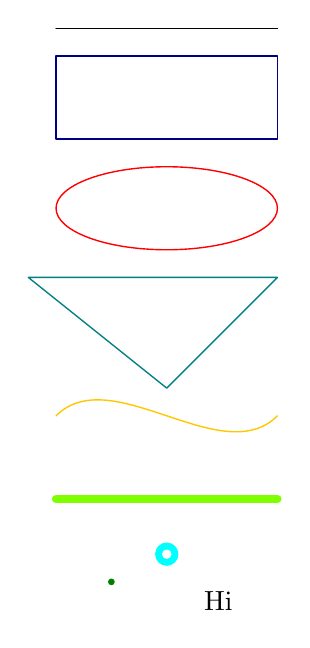
\begin{tikzpicture}[yscale=-1, x=1pt, y=1pt, line join=round, line cap=round]
% Layer color definitions
\definecolor{layer0}{rgb}{0,0,0}
\definecolor{layer1}{rgb}{0,0,0.5}
\definecolor{layer2}{rgb}{1,0,0}
\definecolor{layer3}{rgb}{0,0.5,0.5}
\definecolor{layer4}{rgb}{1,0.78,0}
\definecolor{layer5}{rgb}{0.5,1,0}
\definecolor{layer6}{rgb}{0,1,1}
\definecolor{layer7}{rgb}{0,0.5,0}
\definecolor{layer8}{rgb}{0.6,0.8,0.2}
\definecolor{layer9}{rgb}{1,0.08,0.58}
\definecolor{layer10}{rgb}{0.71,0.61,0.05}
\definecolor{layer11}{rgb}{0,0.5,1}
\definecolor{layer12}{rgb}{0.88,0.88,0.88}
\definecolor{layer13}{rgb}{0.64,0.64,0.64}
\definecolor{layer14}{rgb}{0.37,0.37,0.37}
\definecolor{layer15}{rgb}{0,0,0}
% End of color definitions
\draw[color=layer0, line width=0.5pt] (13,3) -- (93,3);
\node[anchor=north west, color=layer0] at (63,203) {Hi};
\draw[color=layer1, line width=0.5pt] (13,13) rectangle (93,43);
\draw[color=layer2, line width=0.5pt] (53,68) ellipse [x radius=40, y radius=15];
\draw[color=layer3, line width=0.5pt] (13,93) -- (93,93) -- (53,133) -- (3,93) -- cycle;
\draw[color=layer4, line width=0.5pt] (13,143) .. controls (33,123) and (73,163) .. (93,143);
\draw[color=layer5, line width=3pt] (13,173) -- (93,173);
\filldraw[color=layer6] (53,193) ellipse [x radius=4, y radius=4];
\filldraw[color=layer7] (33,203) circle [radius=1];
\filldraw[color=white] (53,193) ellipse [x radius=1.5, y radius=1.5];
\end{tikzpicture}